\section{Strategia}

Il mio periodo di stage \emph{stage} ha avuto luogo parallelamente a una fase di sviluppo del \emph{team} dell'azienda ospitante, relativa al \emph{re-breanding} del sito \emph{e-commerce} 
di un'azienda chiamata \emph{Comfortzone}. Essendo l'azienda ospitante caratterizzata anche da attività di ricerca e sviluppo, l'idea generale è stata quella di 
valutare la possibile integrazione di un sistema intelligente all'interno della loro infrastruttura composta da \emph{e-commerce} e \emph{blog}. 

L'obiettivo strategico identificato dall'azienda è duplice: da un lato migliorare l'esperienza d'uso e la capacità commerciale tramite il loro sito; 
dall'altro sperimentare approcci tecnologici innovativi che possano ridurre le barriere informative per l'utente. 
In questo contesto, lo \emph{stage} è stato pensato non come fine a se stesso, ma come prova di fattibilità (\emph{Proof of Concept}) che potesse alimentare decisioni strategiche successive 
sia in termini di prodotto, sia in termini di processi e competenze interne.

\begin{figure}[htbp]
  \centering
  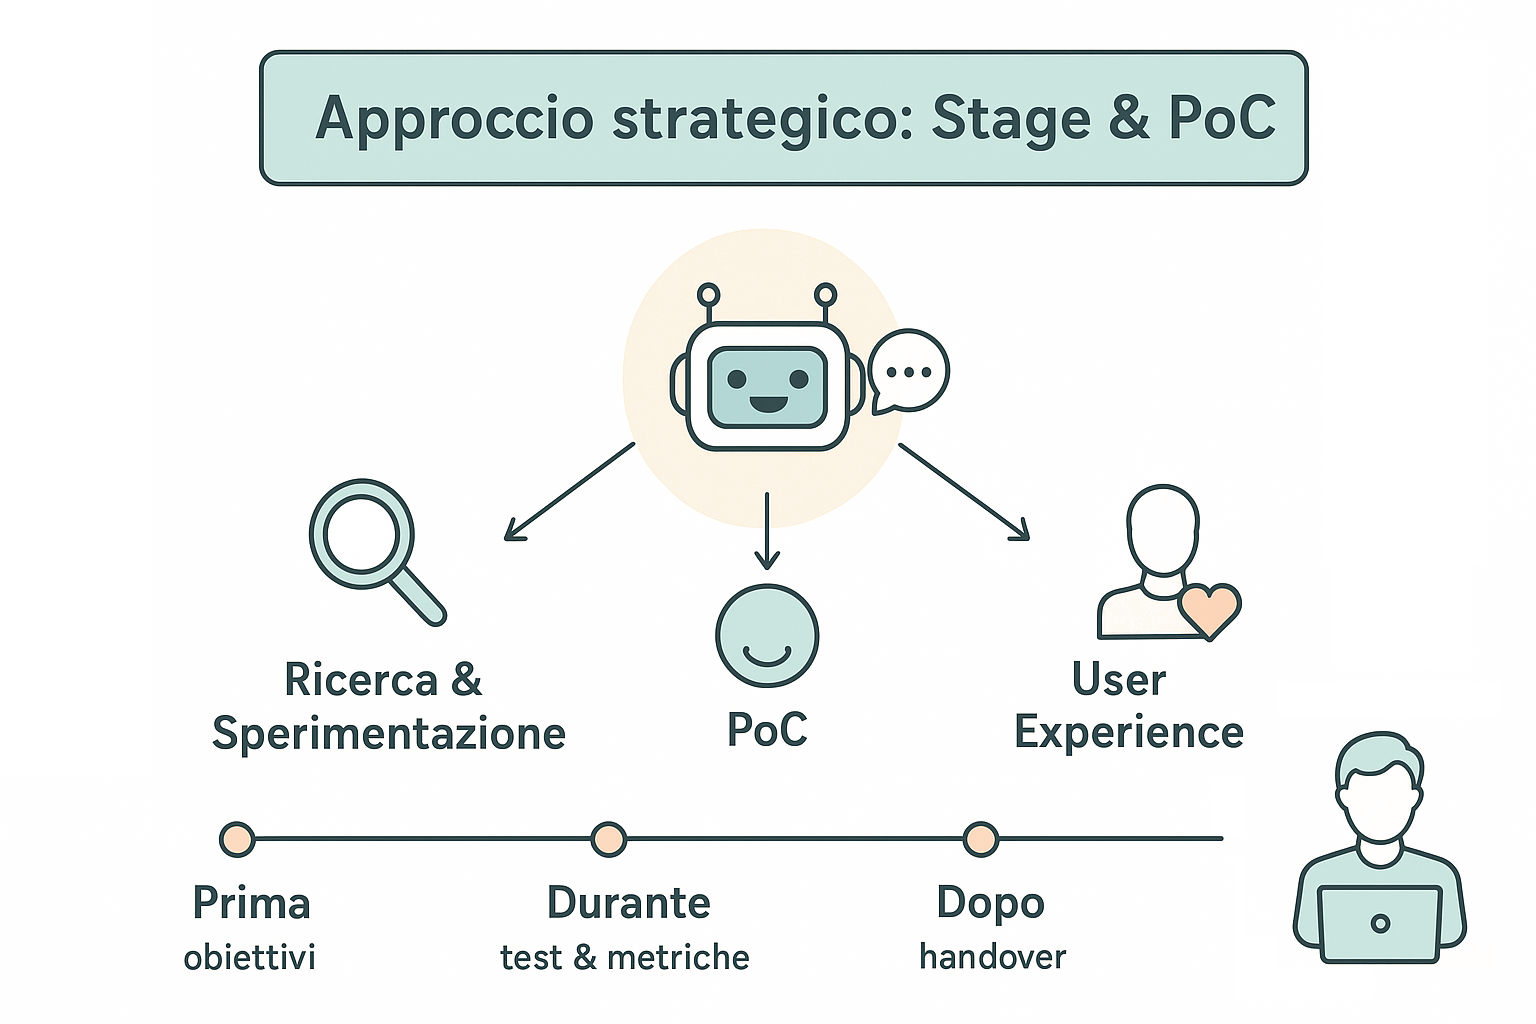
\includegraphics[width=0.8\textwidth]{stage/strategia}
  \caption{Flusso strategico stage.}
  \label{fig:strategia}
\end{figure}

Concretamente, l'organizzazione ospitante ha inteso affrontare i seguenti problemi, attinenti al dominio applicativo della \emph{skin-care} e al canale \emph{e-commerce}:

\begin{itemize}
  \item la complessità informativa per l'utente finale (effetto di \emph{overwelming}), dovuta alla grande quantità di prodotti, varianti e contenuti specialistici presenti sul sito e sul \emph{blog};
  \item la difficoltà di fornire risposte aggiornate, contestuali e personalizzate su brand, prodotti e routine, sfruttando le fonti aziendali (catalogo, schede prodotto, articoli di approfondimento);
  \item la necessità di testare soluzioni tecniche che possano essere integrate rapidamente nell'architettura esistente e che non impediscano una successiva scalabilità o un rapido \emph{deploy}.
\end{itemize}

\begin{figure}[htbp]
  \centering
  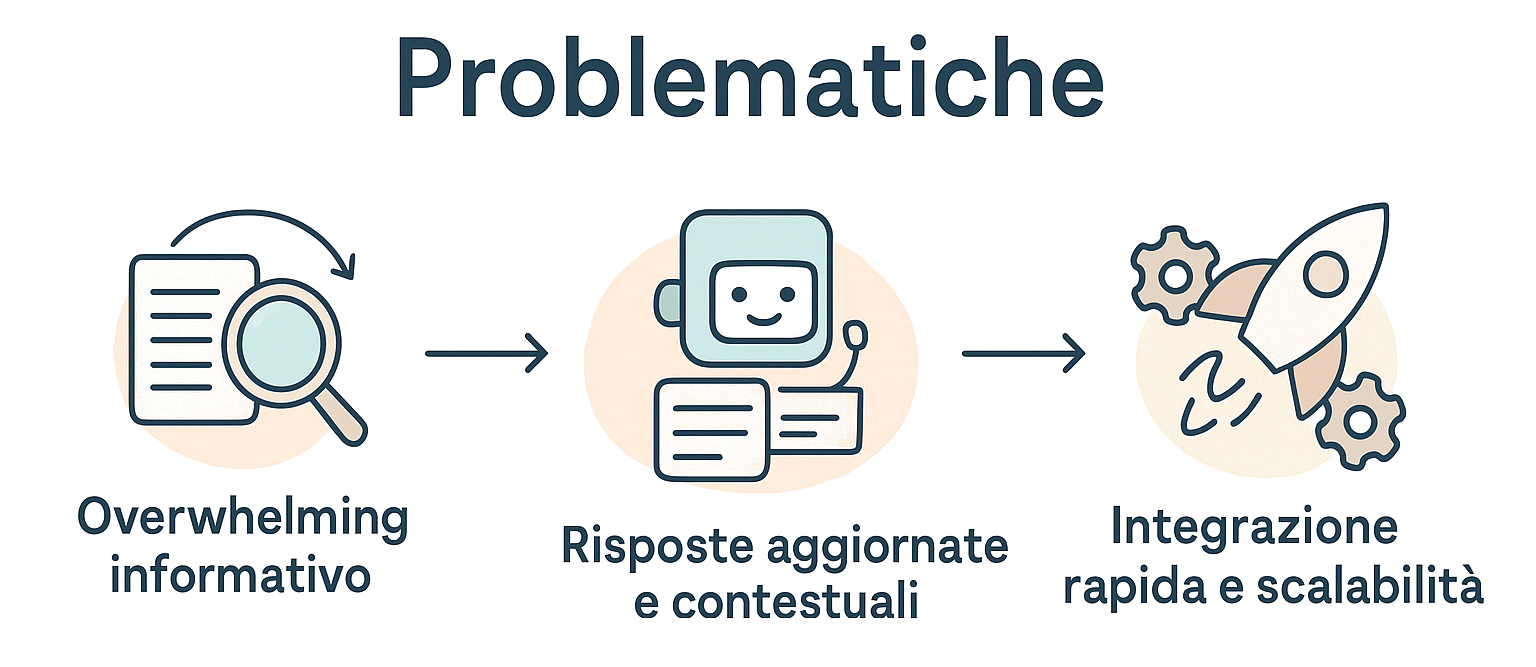
\includegraphics[width=0.8\textwidth]{stage/problematiche}
  \caption{problematiche affrontate attinenti al dominio applicativo.}
  \label{fig:problematiche}
\end{figure}
 
Lo \emph{stage} ha quindi funzionato come un laboratorio sperimentale in cui coniugare ricerca, prototipazione e misurazione: la produzione di un \emph{PoC} non era solo una dimostrazione tecnica, 
ma uno strumento strategico per valutare impatti su conversione, soddisfazione utente e costi operativi.

È importante sottolineare come la proposta di \emph{stage} si collochi all'interno di un ciclo più ampio che precede e segue la sua durata temporale. Prima dello \emph{stage}, 
l'azienda ha definito obiettivi generali di innovazione e ha identificato aree critiche da approfondire; lo \emph{stage} ha permesso di esplorare soluzioni concrete e di mettere 
alla prova ipotesi tecniche. Dopo lo \emph{stage}, i risultati ottenuti (documentazione tecnica, codice del \emph{PoC}, metriche di valutazione, raccomandazioni) 
costituiscono input per fasi successive (ad esempio per ulteriori \emph{stage}), per progetti pilota più estesi o per l'integrazione graduale delle funzionalità in produzione.

Il rapporto dell'azienda con gli \emph{stage} riflette quindi una propensione strutturata all'innovazione: gli \emph{stage} sono visti come strumenti a basso costo per esplorare nuove tecnologie e
formare competenze interne. Questo approccio consente di bilanciare l'accettazione del rischio (esperimenti rapidi e iterativi) 
con la necessità di risultati concretamente sfruttabili nel breve-medio periodo.

Infine, la strategia adottata per il mio \emph{stage} ha privilegiato un orientamento pratico e misurabile: insieme al tutor sono stati definiti indicatori di successo 
(es. tempi di risposta dell'agente, accuratezza delle risposte rispetto alle fonti aziendali, impatto sulla facilità di navigazione e sulla soddisfazione percepita), 
un processo di \emph{handover} (passaggio di consegne o trasferimento di responsabilità tra persone o team) per trasferire tali conoscenza e \emph{assets} al \emph{team}. 
Questi elementi garantiscono che l'attività svolta non resti 
un'esperienza isolata, ma si trasformi in valore duraturo per \emph{Comfortzone} e in una base concreta per interventi successivi.








%Sezione che riporterà come lo stage si inserisce nella visione strategica da parte dell'aziendale (e dunque la  propensione dell’azienda per l’innovazione).
%Qui descriverò parzialmente il punto 2 (perché) riportato nel file Struttura relazione finale.pdf. e lo concluderò nella sezione successiva.


%farlo correggere da chat gpt mantenendo gli inglesismi
%farlo espandere da chatgpt mantenendo gli inglesismi
%creare prompt per immagine illustrative
%togliere sfondo all'immagine
%inserire l'immagine
